\documentclass[tikz,border=7pt]{standalone}
\usepackage{amsmath,amssymb}
\usetikzlibrary{arrows.meta,calc,decorations.pathreplacing,positioning}

% ------------------------------------------------------------
% Three clear schematic TikZ visualizations:
% (1) Gauss map N : M -> S^2
% (2) Differential (dN)_p : T_p M -> T_{N(p)} S^2
% (3) Shape operator S_p = -(dN)_p : T_p M -> T_p M (via identification)
% ------------------------------------------------------------

\begin{document}
	
	% ============================================================
	% (1) Gauss map  N : M -> S^2
	% ============================================================
	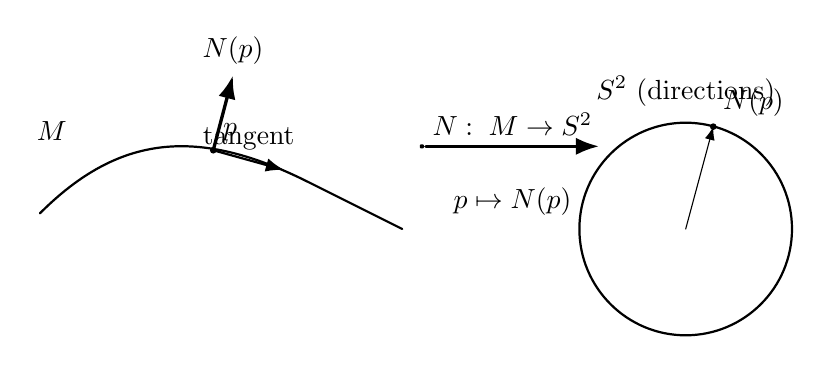
\begin{tikzpicture}[>=Latex, line cap=round, line join=round, scale=1.0]
		
		% --- Left: surface M (schematic curve in a plane) ---
		\begin{scope}[shift={(0,0)}]
			% surface curve
			\draw[thick] (-2.2,0.2) .. controls (-1.2,1.2) and (-0.2,1.3) .. (1.2,0.6)
			.. controls (1.8,0.3) and (2.2,0.1) .. (2.4,0.0);
			\node at (-2.05,1.25) {$M$};
			
			% point p on the surface
			\coordinate (p) at (0,1.0);
			\fill (p) circle (1.2pt) node[above right] {$p$};
			
			% tangent direction at p (small)
			\draw[->,thick] (p) -- ++(0.9,-0.25) node[midway, above] {$\text{tangent}$};
			
			% normal vector N(p)
			\draw[->,very thick] (p) -- ++(0.25,0.95) node[above] {$N(p)$};
		\end{scope}
		
		% --- Right: unit sphere S^2 shown as unit circle (direction space) ---
		\begin{scope}[shift={(6.0,0)}]
			\draw[thick] (0,0) circle (1.35);
			\node at (0,1.75) {$S^2$ (directions)};
			
			% point N(p) on S^2
			\coordinate (np) at (0.35,1.30); % on/near circle for schematic
			\fill (np) circle (1.2pt) node[above right] {$N(p)$};
			
			% radial arrow from origin to N(p)
			\draw[->] (0,0) -- (np);
		\end{scope}
		
		% --- The map arrow N: M -> S^2 ---
		\draw[->,very thick] (2.7,1.05) -- (4.9,1.05) node[midway, above] {$N:\;M\to S^2$};
		\draw[very thick] (2.65,1.05) circle (0.01); % tiny dot for clean arrow start
		
		% --- mapping label p |-> N(p) ---
		\node[align=center] at (3.8,0.35) {$p\mapsto N(p)$};
		
	\end{tikzpicture}
	
	\vspace{10pt}
	
	% ============================================================
	% (2) Differential (dN)_p : T_p M -> T_{N(p)} S^2
	% (computed via curve gamma(t) with gamma(0)=p, gamma'(0)=v)
	% ============================================================
	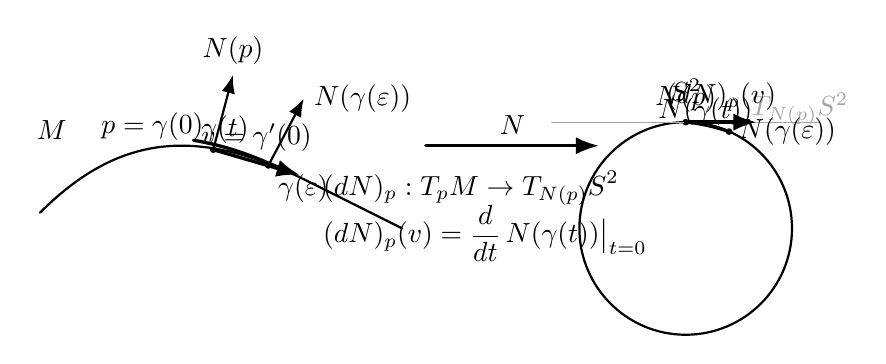
\begin{tikzpicture}[>=Latex, line cap=round, line join=round, scale=1.0]
		
		% --- Left: show curve gamma(t) on M and tangent vector v at p ---
		\begin{scope}[shift={(0,0)}]
			% surface curve M
			\draw[thick] (-2.2,0.2) .. controls (-1.2,1.2) and (-0.2,1.3) .. (1.2,0.6)
			.. controls (1.8,0.3) and (2.2,0.1) .. (2.4,0.0);
			\node at (-2.05,1.25) {$M$};
			
			% choose p and a nearby point q = gamma(eps)
			\coordinate (p) at (0,1.0);
			\coordinate (q) at (0.7,0.8);
			
			\fill (p) circle (1.2pt) node[above left] {$p=\gamma(0)$};
			\fill (q) circle (1.2pt) node[below right] {$\gamma(\varepsilon)$};
			
			% curve segment gamma(t) highlighted
			\draw[very thick] (-0.25,1.12) .. controls (0.15,1.05) and (0.45,0.95) .. (0.95,0.72);
			\node at (0.15,1.25) {$\gamma(t)$};
			
			% tangent vector v = gamma'(0)
			\draw[->,very thick] (p) -- ++(1.1,-0.32) node[midway, above] {$v=\gamma'(0)$};
			
			% normals at p and q
			\draw[->,thick] (p) -- ++(0.25,0.95) node[above] {$N(p)$};
			\draw[->,thick] (q) -- ++(0.45,0.85) node[right] {$N(\gamma(\varepsilon))$};
		\end{scope}
		
		% --- Right: S^2 with point N(p) and tangent space at N(p) ---
		\begin{scope}[shift={(6.0,0)}]
			% unit circle for S^2
			\draw[thick] (0,0) circle (1.35);
			\node at (0,1.75) {$S^2$};
			
			% point N(p) on circle (top-ish)
			\coordinate (np) at (0.0,1.35);
			\fill (np) circle (1.2pt) node[above] {$N(p)$};
			
			% tangent line at N(p): horizontal line
			\draw[gray!70] (-1.7,1.35) -- (1.7,1.35);
			\node[gray!70] at (1.45,1.52) {$T_{N(p)}S^2$};
			
			% small tangent vector (dN)_p(v) at N(p)
			\draw[->,very thick] (np) -- ++(0.9,0) node[midway, above] {$(dN)_p(v)$};
			
			% show that this comes from the curve N(gamma(t)) on S^2
			\coordinate (nq) at (0.55,1.23); % schematic nearby point on circle
			\fill (nq) circle (1.2pt) node[right] {$N(\gamma(\varepsilon))$};
			\draw[very thick] (np) .. controls (0.15,1.34) and (0.35,1.30) .. (nq);
			\node at (0.25,1.48) {$N(\gamma(t))$};
		\end{scope}
		
		% --- Map arrow N and differential arrow (dN)_p ---
		\draw[->,very thick] (2.7,1.05) -- (4.9,1.05) node[midway, above] {$N$};
		
		% Label for differential definition
		\node[align=left] at (3.45,0.15) {%
			$\displaystyle (dN)_p:T_pM\to T_{N(p)}S^2$\\[-1pt]
			$\displaystyle (dN)_p(v)=\frac{d}{dt}\,N(\gamma(t))\big|_{t=0}$};
		
	\end{tikzpicture}
	
	\vspace{10pt}
	
	% ============================================================
	% (3) Shape operator  S_p = -(dN)_p : T_p M -> T_p M
	% via the identification  T_{N(p)}S^2 = (N(p))^\perp = T_p M  in R^3
	% ============================================================
	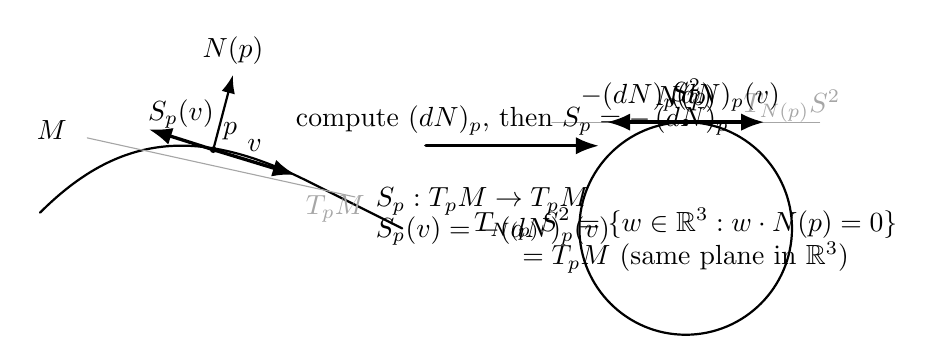
\begin{tikzpicture}[>=Latex, line cap=round, line join=round, scale=1.0]
		
		% --- Left: tangent plane at p (shown as a line) and vectors v and S_p(v) ---
		\begin{scope}[shift={(0,0)}]
			% surface curve M
			\draw[thick] (-2.2,0.2) .. controls (-1.2,1.2) and (-0.2,1.3) .. (1.2,0.6)
			.. controls (1.8,0.3) and (2.2,0.1) .. (2.4,0.0);
			\node at (-2.05,1.25) {$M$};
			
			% point p
			\coordinate (p) at (0,1.0);
			\fill (p) circle (1.2pt) node[above right] {$p$};
			
			% tangent line at p (a local model of T_pM)
			\draw[gray!70] (-1.6,1.15) -- (1.8,0.40);
			\node[gray!70] at (1.55,0.25) {$T_pM$};
			
			% tangent vector v
			\draw[->,very thick] (p) -- ++(1.05,-0.32) node[midway, above] {$v$};
			
			% normal N(p)
			\draw[->,thick] (p) -- ++(0.25,0.95) node[above] {$N(p)$};
			
			% shape operator output S_p(v) = -(dN)_p(v) drawn in the tangent line direction
			\draw[->,very thick] (p) -- ++(-0.82,0.26) node[midway, above] {$S_p(v)$};
		\end{scope}
		
		% --- Right: T_{N(p)}S^2 with (dN)_p(v), then apply minus sign and identify back ---
		\begin{scope}[shift={(6.0,0)}]
			% unit circle for S^2
			\draw[thick] (0,0) circle (1.35);
			\node at (0,1.75) {$S^2$};
			
			% point N(p) at top
			\coordinate (np) at (0,1.35);
			\fill (np) circle (1.2pt) node[above] {$N(p)$};
			
			% tangent line at N(p)
			\draw[gray!70] (-1.7,1.35) -- (1.7,1.35);
			\node[gray!70] at (1.35,1.55) {$T_{N(p)}S^2$};
			
			% (dN)_p(v) at N(p)
			\draw[->,very thick] (np) -- ++(1.0,0) node[midway, above] {$(dN)_p(v)$};
			
			% minus sign: - (dN)_p(v)
			\draw[->,very thick] (np) -- ++(-1.0,0) node[midway, above] {$-(dN)_p(v)$};
			
			% identification note: both tangent spaces are the same plane (orthogonal to N(p))
			\node[align=center] at (0,-0.15) {%
				\(\displaystyle T_{N(p)}S^2=\{w\in\mathbb R^3:w\cdot N(p)=0\}\)\\
				\(\displaystyle =T_pM\) (same plane in \(\mathbb R^3\))};
		\end{scope}
		
		% --- Arrow indicating: use (dN)_p then negate to get shape operator ---
		\draw[->,very thick] (2.7,1.05) -- (4.9,1.05) node[midway, above] {compute $(dN)_p$, then $S_p=-\, (dN)_p$};
		
		% --- Definition block ---
		\node[align=left] at (3.55,0.15) {%
			$\displaystyle S_p:T_pM\to T_pM$\\[-1pt]
			$\displaystyle S_p(v)=-(dN)_p(v)$};
		
	\end{tikzpicture}
	
\end{document}
